% !TEX root = vrptw_terra.tex
% !TEX program = tectonic
% !TEX options = --synctex "%DOC%.tex"
% ============================================================================
% VRPTW-TERRA
% A Heterogeneous Hybrid Routing Framework: Adapting Spatial Indexing
% (Uber H3) and Open-Source Optimization (VROOM/OSM) across Asymmetric
% Indonesian Topographies
% ============================================================================
\documentclass[11pt,a4paper,twocolumn]{article}

% --- Packages ---------------------------------------------------------------
\usepackage[utf8]{inputenc}
\usepackage[T1]{fontenc}
\usepackage{lmodern}
\usepackage[margin=2cm]{geometry}
\usepackage{graphicx}
\usepackage{xcolor}
\usepackage{tikz}
\usetikzlibrary{
  positioning, arrows.meta, shapes.geometric, calc,
  decorations.pathreplacing, decorations.pathmorphing,
  shadows.blur, fit, backgrounds
}
\usepackage{amsmath,amssymb}
\usepackage{booktabs}
\usepackage{enumitem}
\usepackage{hyperref}
\usepackage{float}
\usepackage{fancyhdr}
\usepackage{titlesec}
\usepackage{parskip}
\usepackage{caption}
\raggedbottom
\sloppy
\hbadness=10000
\vbadness=10000
\hfuzz=42pt

% --- Color Palette ----------------------------------------------------------
\definecolor{terraBlue}{HTML}{2563EB}
\definecolor{terraTeal}{HTML}{0D9488}
\definecolor{terraOrange}{HTML}{EA580C}
\definecolor{terraRed}{HTML}{DC2626}
\definecolor{terraGold}{HTML}{D97706}
\definecolor{terraGreen}{HTML}{16A34A}
\definecolor{terraSlate}{HTML}{334155}
\definecolor{terraLight}{HTML}{F1F5F9}
\definecolor{terraPurple}{HTML}{6C3FC5}
\definecolor{seaBlue}{HTML}{0EA5E9}
\definecolor{sandTan}{HTML}{E7D8B0}
\definecolor{hexLow}{HTML}{FEF3C7}
\definecolor{hexMid}{HTML}{FBBF24}
\definecolor{hexHigh}{HTML}{DC2626}

% --- Hyperref Setup ---------------------------------------------------------
\hypersetup{
  colorlinks=true,
  linkcolor=terraBlue,
  citecolor=terraTeal,
  urlcolor=terraTeal,
  pdftitle={When a Jakarta Kilometer Isn't an Ambon Kilometer: Context-Aware Fleet Routing Across Indonesia's Asymmetric Geographies},
  pdfauthor={IT Paragon},
}

% --- Headers & Footers ------------------------------------------------------
\pagestyle{fancy}
\fancyhf{}
\fancyhead[L]{\small\itshape VRPTW-TERRA}
\fancyhead[R]{\small\itshape When a Jakarta Kilometer Isn't an Ambon Kilometer}
\fancyfoot[C]{\small\thepage}
\renewcommand{\headrulewidth}{0.4pt}

% --- Section Title Styling ---------------------------------------------------
\titleformat{\section}
  {\large\bfseries\color{terraSlate}}{\thesection}{0.7em}{}
\titleformat{\subsection}
  {\normalsize\bfseries\color{terraSlate}}{\thesubsection}{0.6em}{}
\titlespacing*{\section}{0pt}{1.1em}{0.5em}
\titlespacing*{\subsection}{0pt}{0.9em}{0.4em}

% --- TikZ Styles -------------------------------------------------------------
\tikzset{
  block/.style={rectangle, rounded corners=2pt, draw=terraSlate!70,
    fill=terraLight, align=center, minimum height=0.85cm,
    font=\small, inner sep=4pt},
  paramblock/.style={rectangle, rounded corners=2pt, draw=terraSlate!70,
    align=center, minimum height=1.0cm, font=\footnotesize, inner sep=3pt},
  decision/.style={diamond, aspect=2.4, draw=terraSlate!70,
    fill=terraGold!15, align=center, font=\small, inner sep=1.5pt},
  arrowline/.style={-{Stealth[length=2.6mm]}, thick, terraSlate},
  outlet/.style={circle, fill=terraBlue, inner sep=1.2pt},
  depotmark/.style={rectangle, fill=terraSlate, inner sep=2.2pt},
}

% Pointy-top hexagon of circumradius #3 centred at (#1,#2), filled with #4
\newcommand{\hexcell}[4]{%
  \draw[draw=terraSlate!55, line width=0.4pt, fill=#4]
    ({#1+#3*cos(30)},{#2+#3*sin(30)}) --
    ({#1+#3*cos(90)},{#2+#3*sin(90)}) --
    ({#1+#3*cos(150)},{#2+#3*sin(150)}) --
    ({#1+#3*cos(210)},{#2+#3*sin(210)}) --
    ({#1+#3*cos(270)},{#2+#3*sin(270)}) --
    ({#1+#3*cos(330)},{#2+#3*sin(330)}) -- cycle;}

% Hexagon on an axial lattice: column #1, row #2, circumradius #3, fill #4
\newcommand{\hexat}[4]{%
  \pgfmathsetmacro{\hx}{(#1 + 0.5*mod(#2,2)) * 1.7320508 * #3}%
  \pgfmathsetmacro{\hy}{#2 * 1.5 * #3}%
  \hexcell{\hx}{\hy}{#3}{#4}}

% ============================================================================
\begin{document}

\twocolumn[{%
  \begin{center}
    {\LARGE\bfseries When a Jakarta Kilometer Isn't an Ambon Kilometer\par}
    \vspace{0.35em}
    {\large Context-Aware Fleet Routing Across Indonesia's
      Asymmetric Geographies\par}
    \vspace{1.1em}
    {\normalsize Arifin Dobson\par}
    {\small IT Paragon --- Enterprise Logistics Research\par}
    {\small \texttt{muhammad.adobson@paracorpgroup.com}\par}
    \vspace{0.4em}
    {\small July 2026\par}
    \vspace{1.2em}
    \begin{minipage}{0.86\textwidth}
      \small
      \textbf{Abstract.}
      Monolithic routing engines systematically underperform in Indonesia
      because the country's operating environments diverge beyond what a
      single parameterization can express: hyper-dense megacities such as
      Jakarta impose extreme node density, congestion-dominated travel
      times, and tight delivery windows, while archipelagic hubs such as
      Ambon impose sparse demand, topographic barriers, and schedule-locked
      maritime crossings. This paper introduces a \emph{Context-Aware
      Parameterization Layer} for an open-source routing stack composed of
      OpenStreetMap (OSM) road data, the OSRM routing engine, the VROOM
      vehicle-routing optimizer, and Uber's H3 hexagonal spatial index. The
      framework classifies a target region into one of two archetypes and
      reconfigures every layer of the stack accordingly: H3 resolution,
      routing profile, and time-window semantics. We formalize the problem
      as a vehicle routing problem with time windows (VRPTW) augmented with
      canvassing coverage rewards, and we inject three physics-inspired
      mechanisms --- a gravitational model of spatial demand for node
      aggregation, simulated annealing for global route search, and a
      topological-viscosity model of effective travel time that unifies
      urban congestion and maritime step delays in a single cost surface.
      We describe the execution pipeline, present the complete mathematical
      formulation, and propose an evaluation protocol contrasting the
      context-aware engine against a monolithic baseline on the
      Jakarta--Ambon archetype pair.
      \par\vspace{0.5em}
      \textbf{Keywords:} vehicle routing, VRPTW, H3 spatial indexing,
      OpenStreetMap, VROOM, gravity model, simulated annealing,
      archipelagic logistics, Indonesia.
    \end{minipage}
    \vspace{1.4em}
  \end{center}
}]

% ============================================================================
\section{Introduction}
\label{sec:intro}

Indonesia is the world's largest archipelagic state: more than 17{,}000
islands spanning three time zones, containing both one of the densest urban
agglomerations on Earth (Greater Jakarta, over 30 million inhabitants) and
some of the most sparsely connected territories in Southeast Asia (Maluku,
Papua). For distribution businesses that combine \emph{delivery} (serving
confirmed orders at exact coordinates) with \emph{canvassing} (dispatching
sales representatives into promising territory to acquire new outlets), this
geography poses a problem that is rarely acknowledged in the routing
literature: the \emph{same} fleet-optimization stack must operate across
regions whose cost structures are not merely different in degree but
different in kind.

A routing engine tuned for Jakarta treats distance as almost irrelevant and
congestion as everything; an engine tuned for Ambon treats congestion as
almost irrelevant and a missed ferry as catastrophic. A single, monolithic
configuration --- one spatial resolution, one routing profile, one
time-window policy --- necessarily fails at least one of these environments.
We refer to this as the \emph{regional divergence problem}.

This paper proposes a remedy that does not require abandoning the
open-source stack that makes nationwide deployment economically viable.
Instead of building separate engines per region, we insert a
\emph{Context-Aware Parameterization Layer} above the stack: a regional
classifier that selects, per territory, (i) the H3 spatial-indexing
resolution used to aggregate demand, (ii) the OSM/OSRM routing profile used
to generate travel-time matrices, and (iii) the constraint semantics
(soft vs.\ hard time windows) passed to the VROOM optimizer.

Our contributions are fourfold:

\begin{enumerate}[leftmargin=1.4em, itemsep=0.15em]
  \item \textbf{A dual-archetype characterization} of Indonesian operating
    environments --- the hyper-dense megacity and the archipelagic hub ---
    with an analysis of the specific failure modes a monolithic engine
    exhibits in each (Section~\ref{sec:archetypes}).
  \item \textbf{A context-aware architecture} that reconfigures each layer
    of the H3/OSM/OSRM/VROOM stack per archetype
    (Section~\ref{sec:architecture}).
  \item \textbf{A unified mathematical formulation} combining a
    VRPTW-with-coverage objective, regional complexity modifiers, and three
    physics-inspired mechanisms: gravitational demand aggregation,
    simulated-annealing route search, and topological viscosity
    (Section~\ref{sec:math}).
  \item \textbf{An evaluation protocol} with explicit hypotheses for
    testing the framework on the Jakarta--Ambon pair against a monolithic
    baseline (Section~\ref{sec:eval}).
\end{enumerate}

The remainder of the paper reviews the underlying technologies
(Section~\ref{sec:background}), develops the archetypes and the
architecture, presents the formulation, describes the execution procedure
and field applications, and closes with limitations and future work.

% ============================================================================
\section{Background and Related Work}
\label{sec:background}

\subsection{Vehicle Routing with Time Windows}

The vehicle routing problem (VRP) originates with Dantzig and
Ramser~\cite{dantzig1959} and generalizes the traveling salesman problem to
fleets with capacity constraints. The time-windowed variant (VRPTW), for
which Solomon~\cite{solomon1987} established the canonical benchmarks,
additionally requires every visit to begin inside a customer-specific
interval. VRPTW is NP-hard; practical solvers rely on construction
heuristics followed by local-search metaheuristics~\cite{toth2014,
braysy2005}. Our formulation extends VRPTW with an \emph{optional-coverage}
term that rewards visiting high-value canvassing territory, placing it in
the family of team-orienteering and prize-collecting VRP variants.

\subsection{The Open-Source Routing Stack}

\textbf{OpenStreetMap (OSM)}~\cite{haklay2008} supplies the underlying road
graph, including attributes critical to this work: \texttt{highway} class,
surface quality, and --- decisive for archipelagic regions ---
\texttt{route=ferry} relations with schedule metadata.
\textbf{OSRM}~\cite{luxen2011} compiles OSM extracts into contraction
hierarchies for millisecond-latency shortest-path and travel-time matrix
queries; its Lua profile mechanism allows the same code base to produce
radically different cost models (car-in-traffic vs.\ ferry-aware).
\textbf{VROOM}~\cite{vroom} consumes those matrices and solves
capacitated VRP/VRPTW instances with a state-of-the-art local-search
pipeline. \textbf{Uber H3}~\cite{brodsky2018} is a hierarchical hexagonal
discrete global grid: at resolution 9 the average cell covers roughly
0.1\,km\(^2\); at resolution 6, roughly 36\,km\(^2\). Hexagons have uniform
neighbor distance and near-isotropic adjacency, making them the natural
aggregation unit for demand surfaces.

\subsection{Gravity Models of Spatial Interaction}

Gravity models --- interaction proportional to the product of masses and
inversely proportional to a power of separation --- have a long lineage in
retail and trade geography, from Reilly's law of retail
gravitation~\cite{reilly1931} through Zipf's intercity-movement
hypothesis~\cite{zipf1946} to Huff's probabilistic trading
areas~\cite{huff1964}. We repurpose this family as a \emph{prioritization
operator} over H3 cells, collapsing thousands of candidate micro-outlets
into a tractable set of weighted centroids.

\subsection{Physics-Inspired Metaheuristics}

Simulated annealing (SA)~\cite{kirkpatrick1983, cerny1985} transplants the
Metropolis acceptance criterion~\cite{metropolis1953} from statistical
mechanics into combinatorial search: worse solutions are accepted with a
probability that decays with a synthetic temperature, allowing early broad
exploration and late greedy refinement. SA remains one of the most robust
metaheuristics for asymmetric, discontinuous cost surfaces --- precisely the
surfaces produced by ferry schedules and rush-hour congestion.

% ============================================================================
\section{The Dual-Archetype Problem}
\label{sec:archetypes}

\begin{figure*}[t]
  \centering
  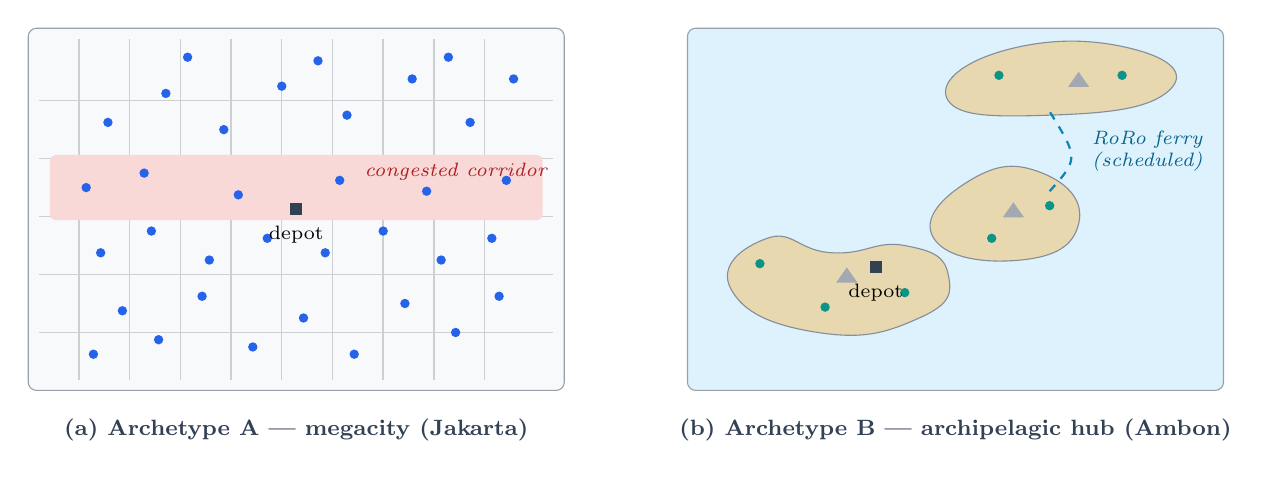
\begin{tikzpicture}[scale=0.92]
    % ---------------- Panel A: Jakarta ----------------
    \begin{scope}
      \draw[terraSlate!50, fill=terraLight!60, rounded corners=3pt]
        (0,0) rectangle (7.4,5.0);
      % street grid
      \foreach \x in {0.7,1.4,...,6.8}
        \draw[terraSlate!25, line width=0.5pt] (\x,0.15) -- (\x,4.85);
      \foreach \y in {0.8,1.6,...,4.4}
        \draw[terraSlate!25, line width=0.5pt] (0.15,\y) -- (7.25,\y);
      % congestion corridor
      \fill[terraRed!18, rounded corners=2pt] (0.3,2.35) rectangle (7.1,3.25);
      \node[font=\scriptsize\itshape, text=terraRed!80!black]
        at (5.9,3.02) {congested corridor};
      % dense outlets
      \foreach \p in {(0.9,0.5),(1.3,1.1),(1.8,0.7),(2.4,1.3),(3.1,0.6),
                      (3.8,1.0),(4.5,0.5),(5.2,1.2),(5.9,0.8),(6.5,1.3),
                      (1.0,1.9),(1.7,2.2),(2.5,1.8),(3.3,2.1),(4.1,1.9),
                      (4.9,2.2),(5.7,1.8),(6.4,2.1),(0.8,2.8),(1.6,3.0),
                      (2.9,2.7),(4.3,2.9),(5.5,2.75),(6.6,2.9),(1.1,3.7),
                      (1.9,4.1),(2.7,3.6),(3.5,4.2),(4.4,3.8),(5.3,4.3),
                      (6.1,3.7),(6.7,4.3),(2.2,4.6),(4.0,4.55),(5.8,4.6)}
        \node[outlet] at \p {};
      \node[depotmark, label={[font=\scriptsize]below:depot}] at (3.7,2.5) {};
      \node[font=\footnotesize\bfseries, text=terraSlate] at (3.7,-0.55)
        {(a) Archetype A --- megacity (Jakarta)};
    \end{scope}
    % ---------------- Panel B: Ambon ----------------
    \begin{scope}[xshift=9.1cm]
      \draw[terraSlate!50, fill=seaBlue!14, rounded corners=3pt]
        (0,0) rectangle (7.4,5.0);
      % main island (two peninsulas joined by an isthmus)
      \draw[terraSlate!60, fill=sandTan]
        plot[smooth cycle, tension=0.9] coordinates
        {(0.6,1.4) (1.8,0.8) (3.2,1.0) (3.6,1.6) (3.0,2.0) (2.0,1.9) (1.1,2.1)};
      \draw[terraSlate!60, fill=sandTan]
        plot[smooth cycle, tension=0.9] coordinates
        {(3.4,2.1) (4.6,1.8) (5.4,2.3) (4.9,3.0) (3.9,2.9)};
      % northern island (Seram)
      \draw[terraSlate!60, fill=sandTan]
        plot[smooth cycle, tension=0.9] coordinates
        {(3.6,4.0) (5.0,3.8) (6.6,4.1) (6.2,4.7) (4.4,4.7)};
      % mountains
      \foreach \p in {(2.2,1.55),(4.5,2.45),(5.4,4.25)}
        \node[isosceles triangle, isosceles triangle apex angle=70,
              rotate=90, fill=terraSlate!45, inner sep=1.6pt] at \p {};
      % ferry route
      \draw[seaBlue!80!black, dashed, thick,
            postaction={decorate}]
        (5.0,2.75) .. controls (5.4,3.2) .. (5.0,3.85);
      \node[font=\scriptsize\itshape, text=seaBlue!60!black, align=left]
        at (6.35,3.3) {RoRo ferry\\(scheduled)};
      % sparse outlets
      \foreach \p in {(1.0,1.75),(1.9,1.15),(3.0,1.35),(4.2,2.1),
                      (5.0,2.55),(4.3,4.35),(6.0,4.35)}
        \node[outlet, fill=terraTeal] at \p {};
      \node[depotmark, label={[font=\scriptsize]below:depot}] at (2.6,1.7) {};
      \node[font=\footnotesize\bfseries, text=terraSlate] at (3.7,-0.55)
        {(b) Archetype B --- archipelagic hub (Ambon)};
    \end{scope}
  \end{tikzpicture}
  \caption{The two operating archetypes. (a)~Jakarta: extreme outlet
    density on a grid-like network where the dominant cost is congestion
    (shaded corridor), not distance. (b)~Ambon: sparse coastal demand,
    topographic barriers (mountains), and inter-island legs that exist only
    as scheduled ferry crossings.}
  \label{fig:archetypes}
\end{figure*}

A monolithic routing engine fails in Indonesia because of \emph{regional
divergence}: the statistical and topological properties that drive routing
cost differ so strongly between regions that any single configuration is
badly mis-tuned for at least one of them. We anchor the analysis in two
diametrically opposed archetypes, illustrated in
Figure~\ref{fig:archetypes}.

\subsection{Archetype A: The Hyper-Dense Megacity (Jakarta)}

Greater Jakarta concentrates tens of thousands of serviceable outlets
(\emph{warung}, minimarkets, modern trade) into a contiguous conurbation.
Its defining properties are: (i)~\textbf{extreme node density} --- hundreds
of candidate visits per square kilometer; (ii)~\textbf{congestion-dominated
travel time} --- the same 5\,km leg can take 12 or 55 minutes depending on
departure time; and (iii)~\textbf{restrictive time windows} --- modern-trade
receiving docks and traffic-restriction schemes impose tight, dense
windows. Distance is a poor proxy for cost; \emph{time-of-day} is the
dominant variable.

\subsection{Archetype B: The Archipelagic Hub (Ambon)}

Ambon and its satellite islands (Seram, Saparua, Haruku) invert every one
of these properties: (i)~\textbf{low node density} --- demand is scattered
across coastal villages (\emph{negeri}) separated by kilometers of empty
road; (ii)~\textbf{linear, topography-constrained networks} --- routes
follow coastlines around mountainous interiors, so the road graph is nearly
one-dimensional and detours are catastrophic; and
(iii)~\textbf{schedule-locked maritime dependencies} --- inter-island legs
exist only at ferry departure times, converting the continuous routing
problem into one punctuated by hard temporal barriers.

\subsection{Failure Modes of a Monolithic Engine}

Applying a single configuration across both archetypes produces four
concrete failure modes:

\begin{enumerate}[leftmargin=1.4em, itemsep=0.15em]
  \item \textbf{Resolution mismatch.} A fine H3 grid (res~9) over Ambon
    yields thousands of empty cells and fragments sparse demand;
    a coarse grid (res~6) over Jakarta merges distinct micro-markets into
    single cells, destroying the density signal canvassing depends on.
  \item \textbf{Profile mismatch.} A car-in-traffic OSRM profile has no
    notion of ferry links or grade resistance, so Ambon inter-island legs
    are either unroutable or assigned absurd travel times; conversely a
    topography profile ignores the rush-hour dynamics that dominate
    Jakarta.
  \item \textbf{Constraint-semantics mismatch.} Soft time windows are
    correct in Jakarta, where a 10-minute tardiness costs goodwill but not
    the route; they are dangerously wrong in Ambon, where missing a ferry
    cut-off strands a vehicle overnight.
  \item \textbf{Cost-surface mismatch.} Jakarta's cost surface is smooth
    but time-varying; Ambon's is piecewise-flat with step discontinuities.
    A solver tuned for one surface explores the other inefficiently.
\end{enumerate}

Table~\ref{tab:parameterization} summarizes the per-archetype
configuration the framework applies to resolve these mismatches.

\begin{table*}[t]
  \centering
  \small
  \caption{Context-aware parameterization of the stack across the two
    archetypes.}
  \label{tab:parameterization}
  \begin{tabular}{@{}p{2.6cm}p{6.4cm}p{6.4cm}@{}}
    \toprule
    \textbf{Component} & \textbf{Archetype A: Jakarta (megacity)} &
      \textbf{Archetype B: Ambon (archipelagic hub)} \\
    \midrule
    Uber H3 resolution &
      High resolution (res 8--9): hexagons of ${\sim}0.1$--$0.7$\,km$^2$
      capture granular store density and neighborhood-level canvassing. &
      Low resolution (res 6--7): hexagons of ${\sim}4$--$36$\,km$^2$ match
      demand scattered thinly across coastal stretches and distinct
      villages (\emph{negeri}). \\
    \addlinespace[0.35em]
    OSM/OSRM routing profile &
      Traffic-heavy profile: time-dependent matrices simulating
      morning/evening rush hours and motorbike lane-splitting behavior. &
      Topographic/ferry profile: slope and surface penalties for steep
      terrain; \texttt{route=ferry} links admitted as valid, schedule-bound
      transit edges. \\
    \addlinespace[0.35em]
    VROOM time windows &
      Soft constraints with buffers: high tardiness penalty, focus on
      dense, rapid sequencing of many small windows. &
      Hard constraints tied to cut-offs: daylight delivery hours, store
      closing times, and immutable ferry departure schedules. \\
    \bottomrule
  \end{tabular}
\end{table*}

% ============================================================================
\section{System Architecture: The Context-Aware Parameterization Layer}
\label{sec:architecture}

\begin{figure}[t]
  \centering
  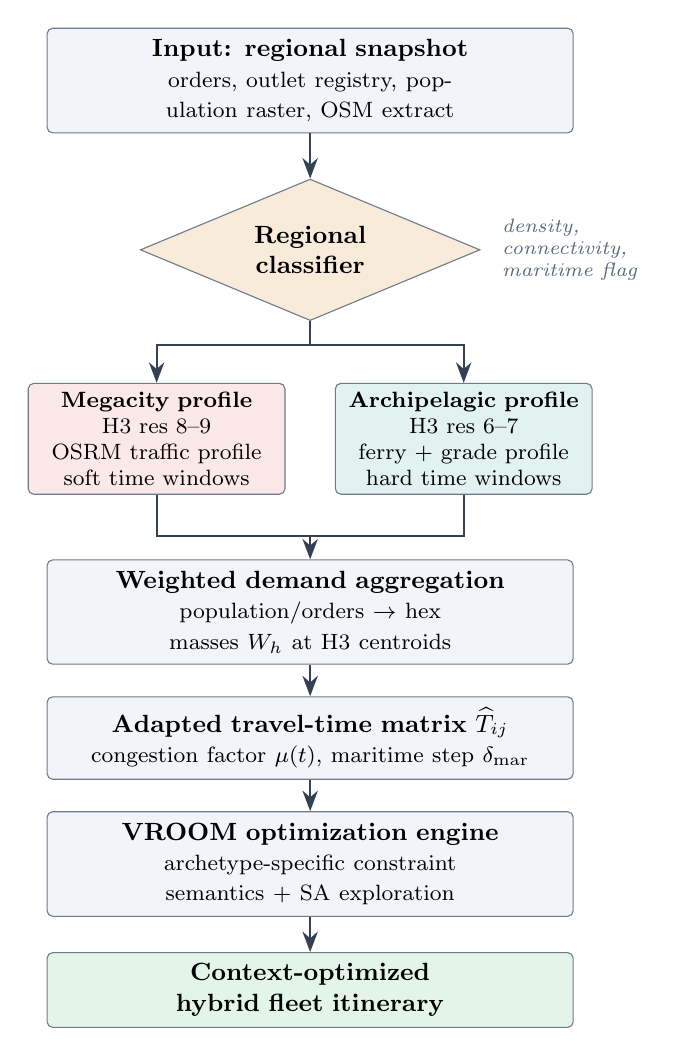
\begin{tikzpicture}
    \node[block, text width=6.4cm] (input) at (0,0)
      {\textbf{Input: regional snapshot}\\
       \footnotesize orders, outlet registry, population raster, OSM extract};
    \node[decision, text width=2.5cm] (classifier) at (0,-2.15)
      {\textbf{Regional\\classifier}};
    \node[paramblock, text width=3.05cm, fill=terraRed!10]
      (profA) at (-1.95,-4.55)
      {\textbf{Megacity profile}\\
       H3 res 8--9\\ OSRM traffic profile\\ soft time windows};
    \node[paramblock, text width=3.05cm, fill=terraTeal!12]
      (profB) at (1.95,-4.55)
      {\textbf{Archipelagic profile}\\
       H3 res 6--7\\ ferry + grade profile\\ hard time windows};
    \node[block, text width=6.4cm] (demand) at (0,-6.75)
      {\textbf{Weighted demand aggregation}\\
       \footnotesize population/orders $\rightarrow$ hex masses $W_h$ at
       H3 centroids};
    \node[block, text width=6.4cm] (matrix) at (0,-8.35)
      {\textbf{Adapted travel-time matrix} $\widehat{T}_{ij}$\\
       \footnotesize congestion factor $\mu(t)$, maritime step
       $\delta_{\mathrm{mar}}$};
    \node[block, text width=6.4cm] (vroom) at (0,-9.95)
      {\textbf{VROOM optimization engine}\\
       \footnotesize archetype-specific constraint semantics +
       SA exploration};
    \node[block, text width=6.4cm, fill=terraGreen!12] (out) at (0,-11.55)
      {\textbf{Context-optimized}\\ \textbf{hybrid fleet itinerary}};
    \draw[arrowline] (input) -- (classifier);
    \coordinate (split) at ($(classifier.south)+(0,-0.30)$);
    \draw[thick, terraSlate] (classifier.south) -- (split);
    \draw[arrowline] (split) -| (profA.north);
    \draw[arrowline] (split) -| (profB.north);
    \coordinate (join) at ($(demand.north)+(0,0.30)$);
    \draw[thick, terraSlate] (profA.south) |- (join);
    \draw[thick, terraSlate] (profB.south) |- (join);
    \draw[arrowline] (join) -- (demand.north);
    \draw[arrowline] (demand) -- (matrix);
    \draw[arrowline] (matrix) -- (vroom);
    \draw[arrowline] (vroom) -- (out);
    \node[font=\scriptsize\itshape, text=terraSlate!80,
          right=0.15cm of classifier, align=left]
      {density,\\ connectivity,\\ maritime flag};
  \end{tikzpicture}
  \caption{Context-aware execution pipeline. The regional classifier
    selects an archetype profile that reconfigures every downstream layer:
    spatial resolution, routing profile, and constraint semantics.}
  \label{fig:pipeline}
\end{figure}

The framework adds one architectural element to the standard
H3/OSM/OSRM/VROOM stack: a \emph{Regional Classifier} that runs before any
matrix generation or optimization, shown in Figure~\ref{fig:pipeline}.

\subsection{Regional Classification}

The classifier consumes three cheap, data-derivable signals:

\begin{itemize}[leftmargin=1.3em, itemsep=0.1em]
  \item \textbf{Demand density} $d$: registered outlets (or historical
    orders) per km$^2$ over the service territory;
  \item \textbf{Network connectivity} $c$: ratio of the largest connected
    road-graph component to total graph size, computed on the OSM extract
    \emph{excluding} ferry edges --- archipelagic regions fragment sharply
    under this test;
  \item \textbf{Maritime dependency flag} $m$: whether any demand lies on a
    component reachable only via \texttt{route=ferry} edges.
\end{itemize}

A territory with high $d$, $c \approx 1$, and $m = 0$ is assigned Archetype
A; low $d$ with $c \ll 1$ or $m = 1$ yields Archetype B. Intermediate
regions (e.g., secondary cities such as Surabaya or Makassar) interpolate
the parameter set; the two archetypes studied here are the calibration
anchors at the extremes.

\subsection{Per-Layer Adaptation}

\textbf{H3 resolution.} The classifier sets the aggregation resolution so
that the \emph{expected demand mass per cell} stays within a target band
--- fine cells in Jakarta preserve micro-market structure; coarse cells in
Ambon avoid fragmenting village-scale demand
(Figure~\ref{fig:hexres}).

\textbf{OSRM profile.} Archetype A compiles a traffic-heavy Lua profile
with time-sliced speed classes per \texttt{highway} tag and a motorbike
variant that discounts congestion (lane-splitting). Archetype B compiles a
topographic profile that penalizes grade and unpaved surfaces and admits
ferry edges with schedule-dependent effective costs.

\textbf{VROOM constraint semantics.} Archetype A submits jobs with soft
time windows (violation penalties in the objective); Archetype B submits
hard windows back-computed from immutable cut-offs --- daylight hours,
store closing times, and ferry departures.

\begin{figure}[t]
  \centering
  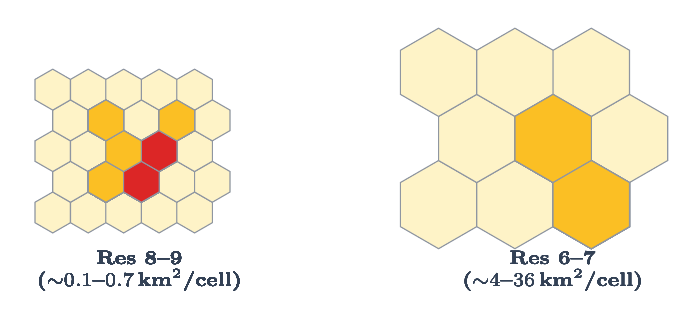
\begin{tikzpicture}
    % ---- fine grid (Jakarta) ----
    \begin{scope}
      \foreach \r in {0,...,4}
        \foreach \c in {0,...,4}
          \hexat{\c}{\r}{0.26}{hexLow}
      % high-demand cells
      \hexat{1}{1}{0.26}{hexMid}
      \hexat{2}{1}{0.26}{hexHigh}
      \hexat{2}{2}{0.26}{hexMid}
      \hexat{3}{2}{0.26}{hexHigh}
      \hexat{3}{3}{0.26}{hexMid}
      \hexat{1}{3}{0.26}{hexMid}
      \node[font=\scriptsize\bfseries, text=terraSlate, align=center]
        at (1.1,-0.75) {Res 8--9\\ (${\sim}0.1$--$0.7$\,km$^2$/cell)};
    \end{scope}
    % ---- coarse grid (Ambon) ----
    \begin{scope}[xshift=4.9cm, yshift=0.1cm]
      \foreach \r in {0,...,2}
        \foreach \c in {0,...,2}
          \hexat{\c}{\r}{0.56}{hexLow}
      \hexat{1}{1}{0.56}{hexMid}
      \hexat{2}{0}{0.56}{hexMid}
      \node[font=\scriptsize\bfseries, text=terraSlate, align=center]
        at (1.45,-0.85) {Res 6--7\\ (${\sim}4$--$36$\,km$^2$/cell)};
    \end{scope}
  \end{tikzpicture}
  \caption{Archetype-dependent H3 resolution. Left: fine hexagons preserve
    Jakarta's micro-market density gradients (darker = higher demand mass
    $W_h$). Right: coarse hexagons match Ambon's village-scale demand
    without fragmenting it.}
  \label{fig:hexres}
\end{figure}

% ============================================================================
\section{Mathematical Formulation}
\label{sec:math}

We now formalize the optimization problem and the three physics-inspired
mechanisms. Table~\ref{tab:notation} collects the notation.

\begin{table}[t]
  \centering
  \small
  \caption{Notation.}
  \label{tab:notation}
  \begin{tabular}{@{}ll@{}}
    \toprule
    \textbf{Symbol} & \textbf{Meaning} \\
    \midrule
    $V$ & set of exact delivery nodes (incl.\ depot) \\
    $H$ & set of H3 canvassing hexagons \\
    $K$ & set of vehicles / sales representatives \\
    $x_{ijk}$ & 1 if vehicle $k$ traverses arc $(i,j)$ \\
    $y_h$ & 1 if hexagon $h$ is canvassed \\
    $C_{ijk}$ & contextual travel cost of arc $(i,j)$ for $k$ \\
    $\rho_h$ & opportunity cost of skipping hexagon $h$ \\
    $W_h$ & demand mass of hexagon $h$ \\
    $\Omega$ & regional complexity factor \\
    $T_{ij}$, $\widehat{T}_{ij}$ & raw / adapted travel time \\
    $\mu(t)$ & time-of-day congestion coefficient \\
    $\delta_{\mathrm{mar}}$ & maritime step delay (wait + processing) \\
    $A_{ij}$ & gravitational attraction toward hexagon $j$ \\
    $M_i, M_j$ & vehicle momentum / hexagon mass \\
    $\nu$ & topological viscosity of the network \\
    $\tau_{\mathrm{disc}}$ & discrete (step) time penalty \\
    $T^{(n)}$ & annealing temperature at iteration $n$ \\
    \bottomrule
  \end{tabular}
\end{table}

\subsection{The Global Objective Function}
\label{sec:objective}

In a hybrid delivery--canvassing network the goal is not merely minimizing
distance: it is \emph{maximizing the value of territory covered} while
respecting rigid time and capacity constraints. We minimize the total cost

\begin{equation}
  \label{eq:objective}
  Z \;=\; \min \Biggl(
    \sum_{i \in V} \sum_{j \in V} \sum_{k \in K} C_{ijk}\, x_{ijk}
    \;+\; \sum_{h \in H} \rho_h \,(1 - y_h)
  \Biggr),
\end{equation}

subject to the standard VRPTW structure. Every mandatory delivery node is
served exactly once,
\begin{equation}
  \sum_{k \in K} \sum_{i \in V} x_{ijk} = 1
  \qquad \forall j \in V \setminus \{0\},
\end{equation}
flow is conserved per vehicle,
\begin{equation}
  \sum_{i \in V} x_{ijk} \;=\; \sum_{i \in V} x_{jik}
  \qquad \forall j \in V,\; \forall k \in K,
\end{equation}
vehicle capacity $Q_k$ is respected,
\begin{equation}
  \sum_{i \in V} \sum_{j \in V} q_j \, x_{ijk} \;\le\; Q_k
  \qquad \forall k \in K,
\end{equation}
and visit times propagate along the adapted travel-time matrix,
\begin{equation}
  \label{eq:timeprop}
  t_{jk} \;\ge\; t_{ik} + s_i + \widehat{T}_{ij}
    - M\,(1 - x_{ijk}),
\end{equation}
where $s_i$ is service duration and $M$ a large constant. Time windows
$[a_j, b_j]$ are enforced with archetype-dependent semantics:
\begin{equation}
  \label{eq:tw}
  \begin{cases}
    \text{soft (A):} &
      Z \mathrel{+}= \sum_{j,k} w_j \max(0,\, t_{jk} - b_j),\\[0.4em]
    \text{hard (B):} &
      a_j \le t_{jk} \le b_j .
  \end{cases}
\end{equation}
A canvassing hexagon counts as covered only if some vehicle actually
enters its centroid node $c(h)$:
\begin{equation}
  y_h \;\le\; \sum_{k \in K} \sum_{i \in V \cup c(H)} x_{i\,c(h)\,k}
  \qquad \forall h \in H.
\end{equation}

Equation~\eqref{eq:objective} creates a deliberate \emph{tension system}:
the solver wants to minimize travel cost $C_{ijk}$ but is penalized
$\rho_h$ for ignoring high-value canvassing territory. The opportunity
cost scales with the hexagon's demand mass, $\rho_h = \eta\, W_h$, with
$\eta$ a business-set conversion rate from demand mass to expected margin.

\subsection{Regional Complexity Modifiers}
\label{sec:modifiers}

The framework refuses to treat an Ambon kilometer like a Jakarta
kilometer. Two modifiers implement this.

\textbf{Demand mass.} Each hexagon's mass composites population $P_h$,
historical order volume $O_h$, and store density $S_h$, scaled by a
regional complexity factor $\Omega_{\mathrm{region}}$:
\begin{equation}
  \label{eq:mass}
  W_h \;=\; \Omega_{\mathrm{region}} \cdot
    \bigl[ \lambda_P P_h + \lambda_O O_h + \lambda_S S_h \bigr],
\end{equation}
where $\lambda_P, \lambda_O, \lambda_S$ are calibration weights.
$\Omega_{\mathrm{region}}$ captures the differential cost of serving a
unit of demand in each region --- effort per rupiah of opportunity is
simply higher in archipelagic territory.

\textbf{Adapted travel time.} The raw OSRM matrix $T_{ij}$ is transformed
into the matrix actually given to the optimizer:
\begin{equation}
  \label{eq:adapted}
  \widehat{T}_{ij} \;=\; T_{ij} \cdot \bigl(1 + \mu(t)\bigr)
    \;+\; \delta_{\mathrm{mar}}(i,j),
\end{equation}
with the congestion coefficient modeled as a baseline plus rush-hour
peaks,
\begin{equation}
  \label{eq:mu}
  \mu(t) = \mu_0
    + A_m e^{-\frac{(t - t_m)^2}{2\sigma_m^2}}
    + A_e e^{-\frac{(t - t_e)^2}{2\sigma_e^2}},
\end{equation}
where $t_m \approx$ 07:00--09:00 and $t_e \approx$ 16:00--19:00 are the
morning and evening peaks. In Jakarta the amplitudes $A_m, A_e$ are large
enough that alternative local-road routing or motorbike dispatch becomes
mandatory during peaks. In Ambon $\mu(t) \approx 0$, but
$\delta_{\mathrm{mar}}$ --- fixed vessel wait plus port processing ---
acts as a heavy step function whenever a route crosses to Seram or
Saparua.

\subsection{Gravitational Aggregation of Spatial Demand}
\label{sec:gravity}

Evaluating $y_h$ against every individual store or prospective customer
makes the coverage subproblem explode combinatorially --- the VRPTW is
already NP-hard, and canvassing multiplies the candidate set by orders of
magnitude. We therefore collapse the demand surface into H3 centroids and
rank them with a \emph{gravitational interaction model}: each hexagon is a
body of mass $W_h$ (written $M_j$ below), and the vehicle experiences an
attraction

\begin{equation}
  \label{eq:gravity}
  A_{ij} \;=\; G\,
    \frac{M_i^{\alpha} \cdot M_j^{\beta}}{\widehat{T}_{ij}^{\;\gamma}},
\end{equation}

where $G$ is a strategic priority constant (raised during, e.g., new
product launches), $M_j$ the target cell's demand mass, $M_i$ the
vehicle's remaining capacity (its ``momentum''), and
$\alpha, \beta, \gamma$ elasticity parameters. Setting $\gamma > 1$
penalizes distant hexagons super-linearly and tightly clusters the
resulting routes --- the spatial analogue of preferring compact orbits.

\begin{figure}[t]
  \centering
  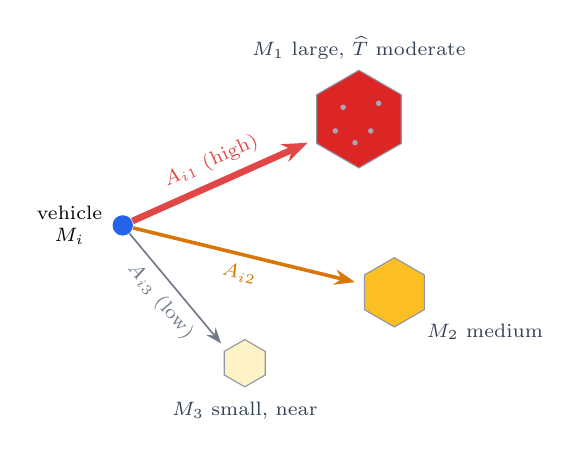
\begin{tikzpicture}[scale=1.0]
    % hexagon masses
    \hexcell{3.0}{1.35}{0.62}{hexHigh}
    \hexcell{3.45}{-0.85}{0.44}{hexMid}
    \hexcell{1.55}{-1.75}{0.30}{hexLow}
    % micro-outlets inside the big hexagon (aggregated away)
    \foreach \p in {(2.8,1.5),(3.15,1.2),(2.95,1.05),(3.25,1.55),(2.7,1.2)}
      \fill[terraSlate!45] \p circle (0.035);
    % vehicle
    \node[circle, fill=terraBlue, inner sep=2.6pt,
          label={[font=\scriptsize, align=center]left:vehicle\\ $M_i$}]
      (veh) at (0,0) {};
    % attraction arrows (width ~ A_ij)
    \draw[-{Stealth[length=3.2mm]}, line width=2.4pt, terraRed!85]
      (veh) -- (2.35,1.05)
      node[midway, above, sloped, font=\scriptsize] {$A_{i1}$ (high)};
    \draw[-{Stealth[length=2.6mm]}, line width=1.3pt, terraGold]
      (veh) -- (2.95,-0.72)
      node[midway, below, sloped, font=\scriptsize] {$A_{i2}$};
    \draw[-{Stealth[length=2.0mm]}, line width=0.6pt, terraSlate!70]
      (veh) -- (1.25,-1.5)
      node[midway, below, sloped, font=\scriptsize] {$A_{i3}$ (low)};
    % mass labels
    \node[font=\scriptsize, text=terraSlate] at (3.0,2.25)
      {$M_1$ large, $\widehat{T}$ moderate};
    \node[font=\scriptsize, text=terraSlate] at (4.6,-1.35)
      {$M_2$ medium};
    \node[font=\scriptsize, text=terraSlate] at (1.55,-2.35)
      {$M_3$ small, near};
  \end{tikzpicture}
  \caption{Gravitational prioritization over H3 centroids. Thousands of
    micro-outlets (small dots) are absorbed into hexagon masses $M_j$; the
    vehicle is pulled toward the highest mass-to-time ratio per
    Eq.~\eqref{eq:gravity}, so only ${\sim}50$ centroid attractions are
    evaluated instead of ${\sim}10^4$ point-to-point routes.}
  \label{fig:gravity}
\end{figure}

\textbf{Efficiency gain.} Instead of computing routes to $10^4$
individual micro-shops, the engine evaluates the pull of ${\sim}50$ H3
centroids (Figure~\ref{fig:gravity}); matrix generation cost falls from
$O(|V_{\mathrm{micro}}|^2)$ to $O((|V| + |H|)^2)$. The vehicle is
mathematically drawn toward clusters with the highest mass-to-distance
ratio, and individual outlets are resolved only \emph{within} a hexagon the
route has already committed to visit.

\subsection{Simulated Annealing for Route Search}
\label{sec:annealing}

Even on the reduced node set, the visit-sequencing landscape over an
asymmetric map is riddled with local minima --- an acceptable loop in
South Jakarta can mask a vastly superior loop through East Jakarta, and in
Ambon a greedy sequence can strand the vehicle on the wrong side of a
ferry cut-off. We therefore drive the improvement phase with simulated
annealing. A temperature $T^{(n)}$ starts high and decays geometrically,
$T^{(n)} = T^{(0)} c^{\,n}$ with $c \in (0.90, 0.99)$, and a candidate
perturbation (2-opt, or-opt, cross-exchange) that changes the cost by
$\Delta E$ is accepted with the Metropolis probability

\begin{equation}
  \label{eq:boltzmann}
  P(\text{accept}) =
  \begin{cases}
    1, & \Delta E < 0, \\[0.4em]
    \exp\!\left( -\dfrac{\Delta E}{k \, T^{(n)}} \right), & \Delta E \ge 0,
  \end{cases}
\end{equation}

with $k$ a scaling constant. While hot, the search deliberately accepts
worse routes and explores broadly across the map; as it cools it locks
into the best basin found (Figure~\ref{fig:annealing}).

\begin{figure}[t]
  \centering
  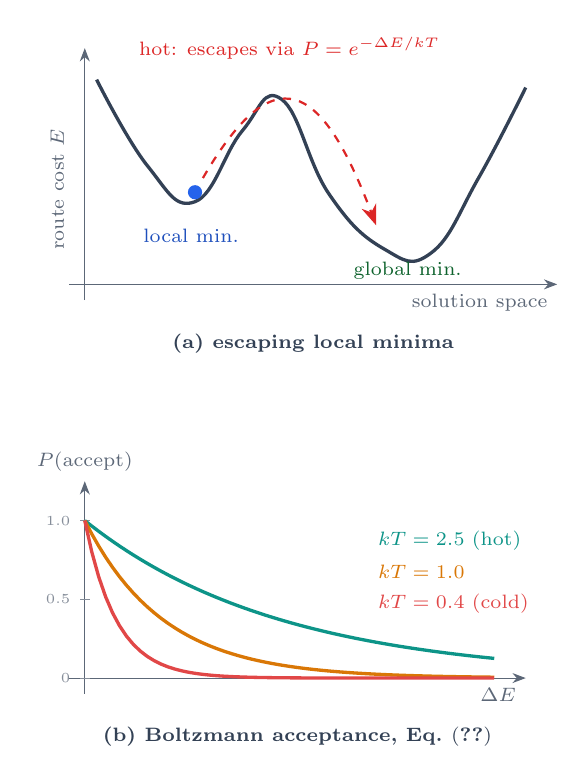
\begin{tikzpicture}[scale=1.0]
    % ---- (a) energy landscape ----
    \draw[-{Stealth}, terraSlate!80] (-0.2,0) -- (6.0,0)
      node[below left, font=\scriptsize] {solution space};
    \draw[-{Stealth}, terraSlate!80] (0,-0.2) -- (0,3.0)
      node[left, font=\scriptsize, rotate=90, yshift=0.35cm,
           xshift=-0.9cm] {route cost $E$};
    \draw[very thick, terraSlate] plot[smooth, tension=0.75] coordinates
      {(0.15,2.6) (0.8,1.5) (1.4,1.05) (2.0,1.95) (2.5,2.35)
       (3.1,1.15) (3.8,0.45) (4.4,0.4) (5.0,1.35) (5.6,2.5)};
    \fill[terraBlue] (1.4,1.17) circle (0.09);
    \node[font=\scriptsize, text=terraBlue!80!black] at (1.35,0.62)
      {local min.};
    \node[font=\scriptsize, text=terraGreen!60!black] at (4.1,0.17)
      {global min.};
    \draw[-{Stealth[length=2.6mm]}, thick, terraRed, dashed]
      (1.5,1.35) .. controls (2.4,2.9) and (3.0,2.6) .. (3.7,0.75);
    \node[font=\scriptsize, text=terraRed] at (2.6,3.0)
      {hot: escapes via $P = e^{-\Delta E / kT}$};
    \node[font=\scriptsize\bfseries, text=terraSlate] at (2.9,-0.75)
      {(a) escaping local minima};
    % ---- (b) acceptance probability ----
    \begin{scope}[yshift=-5.0cm]
      \draw[-{Stealth}, terraSlate!80] (-0.2,0) -- (5.6,0)
        node[below left, font=\scriptsize] {$\Delta E$};
      \draw[-{Stealth}, terraSlate!80] (0,-0.2) -- (0,2.5)
        node[above, font=\scriptsize] {$P(\text{accept})$};
      \foreach \y/\lab in {0/0, 1.0/0.5, 2.0/1.0}
        \draw[terraSlate!60] (0.06,\y) -- (-0.06,\y)
          node[left, font=\tiny] {\lab};
      \draw[very thick, terraTeal, domain=0:5.2, samples=60]
        plot ({\x},{2*exp(-\x/2.5)});
      \draw[very thick, terraGold, domain=0:5.2, samples=60]
        plot ({\x},{2*exp(-\x/1.0)});
      \draw[very thick, terraRed!85, domain=0:5.2, samples=60]
        plot ({\x},{2*exp(-\x/0.4)});
      \node[font=\scriptsize, text=terraTeal, anchor=west] at (3.6,1.75)
        {$kT = 2.5$ (hot)};
      \node[font=\scriptsize, text=terraGold, anchor=west] at (3.6,1.35)
        {$kT = 1.0$};
      \node[font=\scriptsize, text=terraRed!85, anchor=west] at (3.6,0.95)
        {$kT = 0.4$ (cold)};
      \node[font=\scriptsize\bfseries, text=terraSlate] at (2.7,-0.75)
        {(b) Boltzmann acceptance, Eq.~\eqref{eq:boltzmann}};
    \end{scope}
  \end{tikzpicture}
  \caption{Simulated annealing over the routing landscape.
    (a)~At high temperature the search escapes a locally optimal loop
    (e.g., South Jakarta) and discovers a superior basin (a loop including
    East Jakarta). (b)~The probability of accepting a cost increase decays
    with $\Delta E$ and with cooling.}
  \label{fig:annealing}
\end{figure}

\textbf{Efficiency gain.} SA approximates near-optimal tours on both
pathological surfaces --- the discontinuous, ferry-punctuated landscape of
Ambon and the time-varying congestion landscape of Jakarta --- with a
memory footprint linear in route length, which matters for nationwide
batch optimization.

\subsection{Topological Viscosity}
\label{sec:viscosity}

Finally, we unify the two archetypes' cost structures in a single physical
picture: the vehicle does not move through empty space but through a
\emph{medium with viscosity}. Effective travel time on an arc is

\begin{equation}
  \label{eq:viscosity}
  T^{\mathrm{eff}}_{ij} \;=\;
    \frac{D_{ij}}{v_{\mathrm{base}}} \cdot
    \bigl(1 + \nu_{\mathrm{topology}}\bigr)
    \;+\; \tau_{\mathrm{disc}},
\end{equation}

where $D_{ij}$ is arc length, $v_{\mathrm{base}}$ the free-flow speed,
$\nu_{\mathrm{topology}}$ the \emph{continuous} friction of the
environment, and $\tau_{\mathrm{disc}}$ a \emph{discrete} step penalty.
The two archetypes occupy opposite corners of this
$(\nu, \tau)$-space:

\begin{itemize}[leftmargin=1.3em, itemsep=0.1em]
  \item \textbf{Jakarta:} $\nu$ is high and time-varying (live traffic
    density is the dominant friction), while $\tau_{\mathrm{disc}} = 0$
    --- there are no scheduled barriers, only continuous drag.
  \item \textbf{Ambon:} $\nu$ is low but nonzero (road quality, grade),
    while $\tau_{\mathrm{disc}}$ is a massive step barrier --- the RoRo
    ferry wait, which no amount of driving speed can amortize.
\end{itemize}

Figure~\ref{fig:viscosity} visualizes the resulting cumulative-time
profiles. Note that Eq.~\eqref{eq:viscosity} is the arc-level realization
of the matrix transform in Eq.~\eqref{eq:adapted}: $\nu$ implements
$\mu(t)$ plus grade/surface friction, and $\tau_{\mathrm{disc}}$
implements $\delta_{\mathrm{mar}}$. This ensures the optimizer never
``draws lines between coordinates'' --- it evaluates the landscape as a
physical environment with gravity, friction, and thermal state.

\begin{figure}[t]
  \centering
  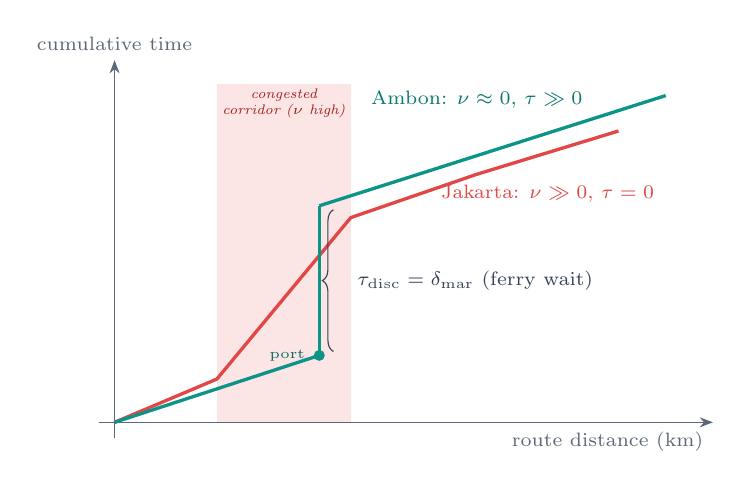
\begin{tikzpicture}[scale=1.0]
    \draw[-{Stealth}, terraSlate!80] (-0.2,0) -- (7.6,0)
      node[below left, font=\scriptsize] {route distance (km)};
    \draw[-{Stealth}, terraSlate!80] (0,-0.2) -- (0,4.6)
      node[above, font=\scriptsize] {cumulative time};
    % congested corridor band (Jakarta)
    \fill[terraRed!12] (1.3,0) rectangle (3.0,4.3);
    \node[font=\tiny\itshape, text=terraRed!75!black, align=center]
      at (2.15,4.05) {congested\\ corridor ($\nu$ high)};
    % Jakarta curve
    \draw[very thick, terraRed!85]
      (0,0) -- (1.3,0.55) -- (3.0,2.6) -- (4.6,3.15) -- (6.4,3.7);
    \node[font=\scriptsize, text=terraRed!85] at (5.5,2.9)
      {Jakarta: $\nu \gg 0$, $\tau = 0$};
    % Ambon curve with ferry step
    \draw[very thick, terraTeal]
      (0,0) -- (2.6,0.85);
    \draw[very thick, terraTeal] (2.6,0.85) -- (2.6,2.75);
    \draw[very thick, terraTeal] (2.6,2.75) -- (7.0,4.15);
    \fill[terraTeal] (2.6,0.85) circle (0.07);
    \node[font=\tiny, text=terraTeal!70!black, left=0.06cm]
      at (2.6,0.85) {port};
    \draw[decorate, decoration={brace, amplitude=4pt}, terraSlate]
      (2.78,0.9) -- (2.78,2.7)
      node[midway, right=0.18cm, font=\scriptsize, text=terraSlate]
      {$\tau_{\mathrm{disc}} = \delta_{\mathrm{mar}}$ (ferry wait)};
    \node[font=\scriptsize, text=terraTeal!80!black] at (4.6,4.1)
      {Ambon: $\nu \approx 0$, $\tau \gg 0$};
  \end{tikzpicture}
  \caption{Topological viscosity, Eq.~\eqref{eq:viscosity}. Jakarta
    accumulates time through continuous friction concentrated in congested
    corridors; Ambon moves through a low-viscosity medium punctuated by a
    step barrier at the ferry crossing.}
  \label{fig:viscosity}
\end{figure}

\subsection{Synthesis: The Contextual Arc Cost}

The arc cost consumed by the objective~\eqref{eq:objective} composes the
pieces above:
\begin{equation}
  C_{ijk} \;=\;
    \phi_t \, T^{\mathrm{eff}}_{ij}(k)
    \;+\; \phi_f \, F_k \, D_{ij},
\end{equation}
where $F_k$ is the fuel/operating rate of vehicle class $k$ (motorbike
vs.\ light truck) and $\phi_t, \phi_f$ convert time and fuel into a common
monetary unit. The gravity scores $A_{ij}$ do not enter $C_{ijk}$
directly; they select \emph{which} hexagon centroids are offered to the
solver as optional high-reward jobs, keeping the instance compact.

% ============================================================================
\section{Context-Aware Execution Procedure}
\label{sec:procedure}

The full pipeline of Figure~\ref{fig:pipeline} executes as follows:

\begin{enumerate}[leftmargin=1.5em, itemsep=0.2em]
  \item \textbf{Classify.} Compute density $d$, connectivity $c$, and
    maritime flag $m$ from the outlet registry and OSM extract; assign the
    archetype and load its parameter profile
    (Table~\ref{tab:parameterization}).
  \item \textbf{Index.} Aggregate population, order history, and store
    registry into H3 cells at the profile's resolution; compute demand
    masses $W_h$ via Eq.~\eqref{eq:mass}.
  \item \textbf{Rank.} Score candidate canvassing cells with the gravity
    model, Eq.~\eqref{eq:gravity}; retain the top-$N$ centroids as
    optional jobs with rewards $\rho_h$.
  \item \textbf{Route the graph.} Compile the archetype's OSRM profile;
    generate the raw matrix $T_{ij}$ over delivery nodes plus retained
    centroids; apply Eq.~\eqref{eq:adapted} to obtain
    $\widehat{T}_{ij}$.
  \item \textbf{Optimize.} Submit jobs, vehicles, capacities, and
    archetype-appropriate time windows (Eq.~\eqref{eq:tw}) to VROOM;
    drive the improvement phase with the annealing schedule of
    Section~\ref{sec:annealing}.
  \item \textbf{Guard.} For Archetype B, back-propagate latest feasible
    departure times from every ferry cut-off and daylight limit along the
    tentative route; if any guard is violated, re-optimize with the
    offending crossing moved to the next scheduled departure or deferred
    to a multi-day loop.
  \item \textbf{Dispatch.} Emit the context-optimized hybrid fleet
    itinerary --- per-vehicle sequences, ETAs, and canvassing targets.
\end{enumerate}

% ============================================================================
\section{Strategic Field Applications}
\label{sec:applications}

\textbf{Jakarta canvassing.} The engine prioritizes high-frequency,
low-payload motorbike sales visits, packing dozens of small time-window
jobs into tight geographic clusters. The gravity exponent $\gamma > 1$
keeps orbits compact; the soft-window penalty of Eq.~\eqref{eq:tw} lets
the solver trade a few minutes of tardiness for substantially denser
sequencing; and the time-sliced matrix steers routes off arterial
corridors during the $\mu(t)$ peaks of Eq.~\eqref{eq:mu}.

\textbf{Ambon canvassing.} The engine plans larger, multi-day loops.
Hard windows anchored to ferry departures and daylight hours ---
propagated backward through Eq.~\eqref{eq:timeprop} --- prevent a vehicle
from being stranded on the far side of the Leitimur or Hitu peninsula or
on Seram after the last crossing. The coarse H3 grid ensures each stop on
a loop represents a village-scale demand mass worth the detour, and
$\Omega_{\mathrm{region}}$ raises $\rho_h$ so that remote-but-strategic
territory is not perpetually starved by the travel-cost term.

\textbf{Fleet composition.} Because $C_{ijk}$ is vehicle-indexed, the same
optimization run allocates motorbikes to dense urban micro-routes and
light trucks to island loops --- the hybrid fleet emerges from the cost
structure rather than being hand-assigned.

% ============================================================================
\section{Proposed Evaluation Protocol}
\label{sec:eval}

The framework is designed for empirical validation on the archetype pair.
We propose the following protocol.

\textbf{Data.} OSM extracts for DKI Jakarta and Maluku (Geofabrik);
outlet registries and historical order volumes from distributor records;
population rasters for $P_h$; published ferry schedules for the
Ambon--Seram and Ambon--Saparua crossings.

\textbf{Baseline.} The identical stack with a single monolithic
configuration --- H3 res~8, default OSRM car profile, uniform soft time
windows --- applied to both regions.

\textbf{Scenarios.} Matched daily instances per region: delivery-only,
canvassing-only, and hybrid; weekday vs.\ weekend traffic in Jakarta;
single-day vs.\ multi-day loops in Ambon.

\begin{table}[t]
  \centering
  \small
  \caption{Evaluation metrics.}
  \label{tab:metrics}
  \begin{tabular}{@{}ll@{}}
    \toprule
    \textbf{Metric} & \textbf{Captures} \\
    \midrule
    Total route duration & efficiency \\
    On-time arrival rate & window fidelity \\
    Ferry cut-off violations & stranding risk (B) \\
    Weighted coverage $\frac{\sum_h W_h y_h}{\sum_h W_h}$ & canvassing value \\
    Matrix + solve wall-time & tractability \\
    Vehicle-km per served demand unit & cost intensity \\
    \bottomrule
  \end{tabular}
\end{table}

\textbf{Hypotheses.}
\begin{itemize}[leftmargin=2.6em, itemsep=0.1em]
  \item[\textbf{H1.}] In Jakarta, the context-aware engine improves
    on-time arrival rate and weighted coverage at equal fleet size, by
    exploiting time-sliced matrices and fine-grained hexagon masses.
  \item[\textbf{H2.}] In Ambon, the context-aware engine reduces ferry
    cut-off violations to zero while the monolithic baseline either
    strands vehicles or defensively under-serves outer islands.
  \item[\textbf{H3.}] Gravitational aggregation reduces matrix-generation
    and solve wall-time by at least an order of magnitude relative to
    routing all micro-outlets, at negligible loss in realized coverage
    value.
\end{itemize}

% ============================================================================
\section{Discussion and Limitations}
\label{sec:discussion}

\textbf{Data freshness.} OSM coverage in eastern Indonesia is thinner and
less frequently edited than in Java; grade and surface tags are
incomplete, which degrades the Archetype-B viscosity term. Field GPS
traces can progressively correct the profile.

\textbf{Schedule volatility.} Ferry timetables in Maluku shift with
weather and season; $\delta_{\mathrm{mar}}$ must be treated as a
distribution, not a constant, and the guard step of
Section~\ref{sec:procedure} should plan against a conservative quantile.

\textbf{Calibration burden.} The elasticities
$(\alpha, \beta, \gamma)$, mass weights
$(\lambda_P, \lambda_O, \lambda_S)$, and
$\Omega_{\mathrm{region}}$ require historical conversion data to fit;
until then they are expert-set priors. Sensitivity analysis over these
parameters belongs in the evaluation protocol.

\textbf{Classifier granularity.} The two-archetype dichotomy is a
deliberate simplification. Secondary cities blend both regimes; the
parameter layer supports interpolation, but the interpolation policy
itself is future work.

\textbf{Stochasticity.} SA is nondeterministic; production deployments
should fix seeds per planning run and report cost distributions, not
single draws.

% ============================================================================
\section{Conclusion}
\label{sec:conclusion}

We presented VRPTW-TERRA, a heterogeneous hybrid routing framework that
adapts an entirely open-source stack --- OSM, OSRM, VROOM, and Uber H3 ---
to the extreme regional divergence of Indonesian logistics. Rather than
building per-region engines, the framework inserts a Context-Aware
Parameterization Layer that classifies a territory and reconfigures
spatial resolution, routing profile, and constraint semantics in one
motion. A unified formulation couples a VRPTW-with-coverage objective to
three physics-inspired mechanisms: gravitational demand aggregation that
collapses intractable canvassing sets into weighted hexagon centroids,
simulated annealing that survives the discontinuous cost surfaces of
archipelagic geography, and a topological-viscosity model that expresses
Jakarta's congestion and Ambon's ferry barriers as two corners of the same
$(\nu, \tau)$ space. The result is an engine that treats the landscape as
a physical environment --- with gravity, friction, and thermal state ---
rather than as empty space between coordinates. Empirical validation on
the Jakarta--Ambon pair, per the protocol of Section~\ref{sec:eval}, is
the immediate next step.

% ============================================================================
\begin{thebibliography}{9}
\small

\bibitem{dantzig1959}
G.~B. Dantzig and J.~H. Ramser,
``The Truck Dispatching Problem,''
\emph{Management Science}, vol.~6, no.~1, pp.~80--91, 1959.

\bibitem{solomon1987}
M.~M. Solomon,
``Algorithms for the Vehicle Routing and Scheduling Problems with Time
Window Constraints,''
\emph{Operations Research}, vol.~35, no.~2, pp.~254--265, 1987.

\bibitem{toth2014}
P.~Toth and D.~Vigo, Eds.,
\emph{Vehicle Routing: Problems, Methods, and Applications}, 2nd~ed.
Philadelphia, PA: SIAM, 2014.

\bibitem{braysy2005}
O.~Br{\"a}ysy and M.~Gendreau,
``Vehicle Routing Problem with Time Windows, Part~I: Route Construction
and Local Search Algorithms,''
\emph{Transportation Science}, vol.~39, no.~1, pp.~104--118, 2005.

\bibitem{kirkpatrick1983}
S.~Kirkpatrick, C.~D. Gelatt, and M.~P. Vecchi,
``Optimization by Simulated Annealing,''
\emph{Science}, vol.~220, no.~4598, pp.~671--680, 1983.

\bibitem{cerny1985}
V.~{\v C}ern{\'y},
``Thermodynamical Approach to the Traveling Salesman Problem: An
Efficient Simulation Algorithm,''
\emph{Journal of Optimization Theory and Applications}, vol.~45,
pp.~41--51, 1985.

\bibitem{metropolis1953}
N.~Metropolis, A.~W. Rosenbluth, M.~N. Rosenbluth, A.~H. Teller, and
E.~Teller,
``Equation of State Calculations by Fast Computing Machines,''
\emph{Journal of Chemical Physics}, vol.~21, no.~6, pp.~1087--1092, 1953.

\bibitem{brodsky2018}
I.~Brodsky,
``H3: Uber's Hexagonal Hierarchical Spatial Index,''
Uber Engineering Blog, 2018.
[Online]. Available: \url{https://www.uber.com/blog/h3/}

\bibitem{luxen2011}
D.~Luxen and C.~Vetter,
``Real-Time Routing with OpenStreetMap Data,''
in \emph{Proc.\ 19th ACM SIGSPATIAL Int.\ Conf.\ on Advances in
Geographic Information Systems}, 2011, pp.~513--516.

\bibitem{vroom}
J.~Coupey, J.-M. Nicod, and C.~Varnier,
\emph{VROOM: Vehicle Routing Open-source Optimization Machine}, Verso.
[Online]. Available: \url{http://vroom-project.org/}

\bibitem{haklay2008}
M.~Haklay and P.~Weber,
``OpenStreetMap: User-Generated Street Maps,''
\emph{IEEE Pervasive Computing}, vol.~7, no.~4, pp.~12--18, 2008.

\bibitem{reilly1931}
W.~J. Reilly,
\emph{The Law of Retail Gravitation}.
New York, NY: Knickerbocker Press, 1931.

\bibitem{zipf1946}
G.~K. Zipf,
``The $P_1 P_2 / D$ Hypothesis: On the Intercity Movement of Persons,''
\emph{American Sociological Review}, vol.~11, no.~6, pp.~677--686, 1946.

\bibitem{huff1964}
D.~L. Huff,
``Defining and Estimating a Trading Area,''
\emph{Journal of Marketing}, vol.~28, no.~3, pp.~34--38, 1964.

\end{thebibliography}

\end{document}
